% ============================================================
%  chapter02g_kolmogorov_complexity_slides.tex
%  Chapter 2: Background -- Section 2.7 Kolmogorov Complexity
%  An Introduction to Universal Artificial Intelligence
%  Hutter, Quarel & Catt --- CRC Press, 2024
% ============================================================
\documentclass[aspectratio=169,10pt]{beamer}

\usetheme{Madrid}
\usecolortheme{seahorse}
\usefonttheme{professionalfonts}

% -- packages ------------------------------------------------------------------
\usepackage{amsmath,amssymb,bm}
\usepackage{graphicx}
\usepackage{booktabs}
\usepackage{listings}
\usepackage{xcolor}
\usepackage{tikz}
\usetikzlibrary{shapes,arrows,positioning,calc}
\usepackage{mathtools}
\usepackage{array}
\usepackage{multirow}
\usepackage{makecell}

\graphicspath{{figures/}}

% -- listings style --------------------------------------------------------
\lstdefinestyle{pythonstyle}{
  language=Python,
  basicstyle=\ttfamily\scriptsize,
  keywordstyle=\color{blue}\bfseries,
  stringstyle=\color{orange},
  commentstyle=\color{green!50!black}\itshape,
  numberstyle=\tiny\color{gray},
  numbers=left,
  stepnumber=1,
  numbersep=5pt,
  frame=single,
  backgroundcolor=\color{gray!7},
  breaklines=true,
  showstringspaces=false,
  tabsize=2,
  captionpos=b,
}
\lstset{style=pythonstyle}

% -- beamer setup -----------------------------------------------------------
\setbeamertemplate{footline}[frame number]
\setbeamertemplate{navigation symbols}{}
\setbeamersize{text margin left=0.5cm, text margin right=0.5cm}

% -- convenient macros -------------------------------------------------------
\newcommand{\Bstr}{\mathbb{B}^*}
\newcommand{\explain}[1]{\par\smallskip{\footnotesize\itshape #1}\par}

% -- title -------------------------------------------------------------------
\title[UAI -- Ch.2.7 Kolmogorov Complexity]{An Introduction to Universal Artificial Intelligence}
\subtitle{Chapter 2 (Background): Section 2.7 -- Kolmogorov Complexity}
\author{Based on Hutter, Quarel \& Catt}
\institute{CRC Press, 2024}
\date{}

% =============================================================================
\begin{document}
% =============================================================================

\begin{frame}
  \titlepage
\end{frame}

\begin{frame}{Outline}
  \tableofcontents
\end{frame}

% =============================================================================
\section{2.7.1 Motivation}
% =============================================================================

\begin{frame}[allowframebreaks]{From Shannon Entropy to a Complexity of Individual Objects}
  In Section 2.5 we introduced \textbf{Shannon entropy}, which measures the
  \emph{expected} information of a stochastic source -- that is, the expected
  number of bits required to encode a string sampled from a distribution
  $P$. Entropy is a property of a random variable / distribution, not of any
  single outcome.

  \medskip
  A different notion of information measures the intrinsic information
  contained in \emph{a single message itself}, rather than the
  unpredictability of the source that produced it: this is the
  \textbf{Kolmogorov complexity}. It is a property of one particular string,
  defined as the length of the shortest description of that string.

  \bigskip
  \textbf{Intuition.} The Kolmogorov complexity of a string represents the
  length of the shortest possible \emph{compressed} form of that string. It
  can therefore be used as a formal measure of the simplicity/complexity of
  any object that can be encoded as a string, using Turing machines
  (Definition 2.6.2) as the reference language for ``descriptions'' -- just
  as we did for computability theory in Section 2.6.

  \framebreak

  \textbf{Why we care.} Kolmogorov complexity gives a rigorous meaning to
  ``simplicity'', which lets us favor simple explanations of data (Occam's
  razor) in a principled way. Many properties of Kolmogorov complexity have
  a direct analogue in Shannon entropy (we will build a full comparison
  table later, Table 2.20). One key difference: Kolmogorov complexity is
  \textbf{not finitely computable} -- there provably cannot exist an
  algorithm that outputs it exactly (Theorem 2.7.27). This means we can
  never compute the \emph{exact} Kolmogorov complexity of an object in
  practice, but it still gives a useful theoretical underpinning for
  simplicity, on which universal predictors (like AIXI, in later chapters)
  can be built. Given enough time, $K$ \emph{can} be approximated
  arbitrarily well from above (Theorem 2.7.28), and any practical data
  compressor gives an upper bound on the true Kolmogorov complexity of an
  object.
\end{frame}

\begin{frame}{Three Strings, Same Length: Which Is ``Simple''?}
  \footnotesize
  Consider the following three binary strings, each 40 bits long:
  \begin{align*}
    x &= 1010101010101010101010101010101010101010\\
    y &= 1100100100001111110110101010001000100001\\
    z &= 1011101100110101111100011101011010111011000
  \end{align*}
  \vspace{-0.3em}
  \begin{itemize}\itemsep0pt
    \item $x$ has an obvious simple pattern: the pair \texttt{10} repeated
      twenty times.
    \item $y$ at first glance looks ``random,'' but is actually the first
      40 bits of the binary expansion of $\pi$ (pi).
    \item $z$ was generated by measuring quantum fluctuations of a vacuum
      -- as far as we can tell truly random: given all past bits, we
      cannot predict the next bit with more than 50\% accuracy.
  \end{itemize}
  \begin{center}
    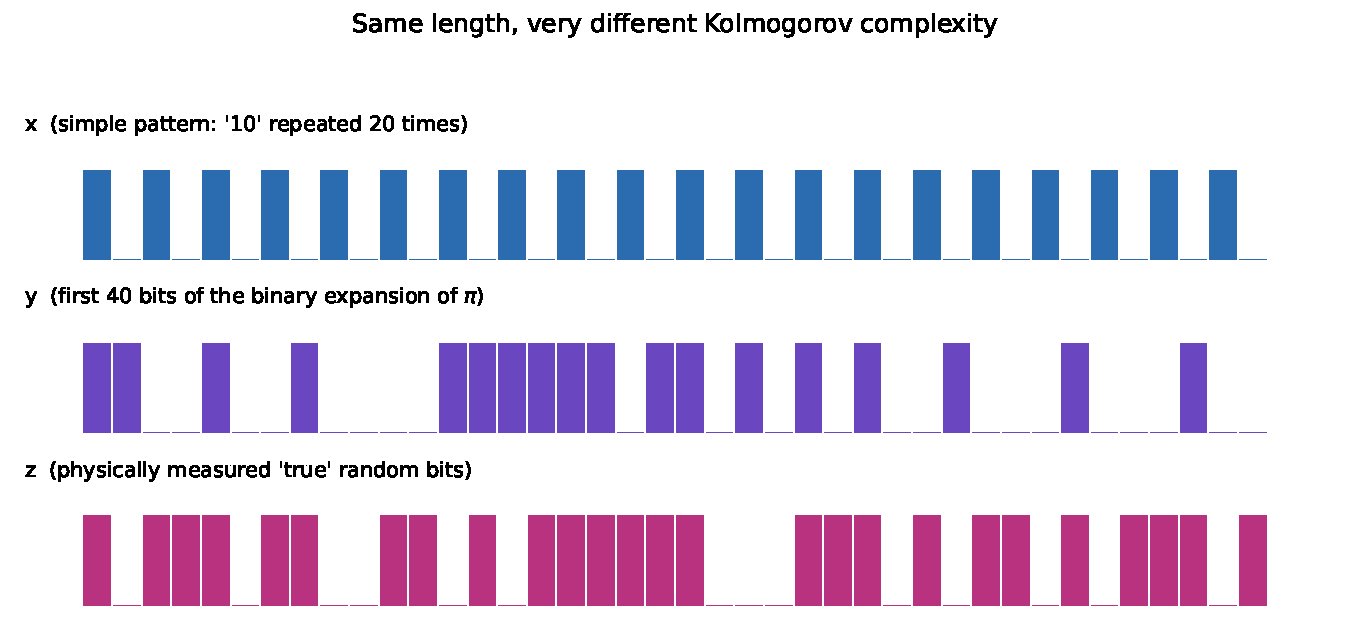
\includegraphics[width=0.5\linewidth]{three_strings}
  \end{center}
\end{frame}

\begin{frame}[allowframebreaks]{What Makes a String ``Simple''?}
  \textbf{Ease of prediction is not quite the right notion.} One could
  argue simplicity is about the ease with which the next bit can be
  predicted: for $x$, after observing only a few bits we can spot the
  pattern and predict the rest perfectly (this notion of complexity via
  difficulty of prediction was explored by Legg and Hutter). However, $y$
  (the digits of $\pi$) certainly appears to have no clear pattern, and
  will pass most statistical tests for randomness. Yet if we knew ahead of
  time that $y$ was just the binary expansion of $\pi$, we could predict
  every future bit perfectly by computing $\pi$ to the required precision.
  So it \emph{is} possible to predict both $x$ and $y$ perfectly, yet
  intuitively $x$ still feels simpler than $y$.

  \bigskip
  \textbf{The right notion: length of description.} The difference lies in
  the \emph{length of the description}. We can describe $x$ as ``repeat 10
  twenty times'' and $y$ as ``the binary expansion of
  $4\sum_{i=0}^{\infty}(-1)^i/(2i+1)$ to 40 bits.'' Had we taken longer
  continuations of $x$ and $y$ (a few thousand bits), the description of
  each would stay roughly the same length, vastly smaller than the string
  itself. These sequences are simple because they are
  \emph{compressible}. This is (probably) not true for $z$, whose
  shortest description is plausibly the string itself.

  \framebreak

  \textbf{Many ways to describe the same object.} There are many other ways
  to describe $\pi$, of wildly different lengths depending on what
  background knowledge is assumed:
  \begin{itemize}
    \item As an integral: $\displaystyle \pi = 4\int_0^1 \sqrt{1-x^2}\,dx$.
    \item As a limiting geometric process: inscribe regular $n$-sided
      polygons in a circle of radius 1 and calculate their area as
      $n\to\infty$.
    \item As a description that uniquely identifies $\pi$ (the ratio of a
      circle's circumference to its diameter) while omitting entirely how
      to compute it.
  \end{itemize}
  To someone missing the relevant mathematical background, any of these
  descriptions may take several pages (defining what addition, an
  integral, or a limit even means). The simplicity of a description
  therefore depends on \emph{who you are talking to}.

  \framebreak

  \textbf{The fix: a fixed universal interpreter.} We need a fixed,
  universally agreed-upon interpreter that takes ``descriptions'' (i.e.\
  programs) and returns the sequence described. Such a machine should be
  unbiased towards any particular class of sequences, to avoid the
  problems above (which language? which symbols are permitted? does the
  decoder already know calculus?).

  \medskip
  Note that entropy (Definition 2.5.1) is unhelpful here as a notion of
  ``simplicity''/``information content'': any deterministic process always
  has zero bits of entropy, so a machine that prints the digits of $\pi$
  would have zero entropy despite being an interesting, structured object.
  We are instead concerned with a definition that relates to the
  \emph{intrinsic} information contained in an individual object -- the
  minimal quantity of information required to reconstruct it. Turing
  machines (Definition 2.6.2) will play the role of this fixed, universal
  interpreter.
\end{frame}

% =============================================================================
\section{2.7.2 Making Simplicity Rigorous}
% =============================================================================

\begin{frame}{Turing Machines as the Universal Description Interpreter}
  \textbf{Turing machines} (Definition 2.6.2) provide an ideal model for a
  description interpreter: assuming the Church--Turing thesis (Thesis
  2.6.6), for any algorithm that generates a sequence there exists a Turing
  machine that implements that algorithm.

  \medskip
  For technical reasons we need two specific variants of a Turing machine
  that read their input/output in a one-directional (streaming) fashion.
\end{frame}

\begin{frame}[allowframebreaks]{Definition 2.7.1: Prefix / Monotone Turing Machine}
  \begin{block}{Definition 2.7.1 (Prefix/Monotone Turing Machine)}
    A prefix/monotone Turing machine is a Turing machine with one
    unidirectional input tape, one unidirectional output tape, and some
    bidirectional work tapes. Input tapes are read only, output tapes are
    write only, and unidirectional tapes are those where the head can only
    move from left to right. All tapes are binary (no blank symbol), work
    tapes are initialized with zeros.

    \textbf{Prefix TM.} We say $T$ halts on input $p$ with output $x$, and
    write $T(p)=x$ if $p$ is to the left of the input head and $x$ is to
    the left of the output head after $T$ halts. The set of $p$ on which
    $T$ halts forms a \emph{prefix code}. We call such codes $p$
    \emph{self-delimiting} programs.

    \textbf{Monotone TM.} We say $T$ outputs/computes a string starting
    with $x$ (or an infinite sequence $\omega$) on input $p$, and write
    $T(p)=x*$ (or $T(p)=\omega$) if $p$ is to the left of the input head
    when the last bit of $x$ is output ($T$ reads all of $p$ but no more,
    and for every $N$ there exists a time step $t_0$ such that for all
    $t\ge t_0$, the output tape is prefixed with $\omega_{1:N}$). $T$ may
    continue operating and need not halt (must not halt for infinite
    sequences). For a given $x$, the set of such programs $p$ forms a
    prefix code. We call such codes $p$ \emph{minimal} programs.
  \end{block}

  \explain{Plain English: a prefix Turing machine reads a self-contained
  program $p$ bit by bit (never reading past the end of $p$, since it
  halts before that), and outputs a finite string $x$. A monotone Turing
  machine is similar, but is allowed to keep running forever and produce
  an ever-growing (never-retracted) output, which is useful for describing
  infinite sequences $\omega$. ``Prefix code'' means no valid program is a
  prefix of another valid program -- this is what lets the machine know,
  just from reading bits one at a time, exactly when a program ends.}
\end{frame}

\begin{frame}[allowframebreaks]{Definition 2.7.2: Universal Turing Machine (UTM)}
  Any Turing machine $T$ can be expressed as a single binary string
  $\langle T\rangle$ in some canonical way, such that all defining
  properties of $T$ can be recovered from $\langle T\rangle$. By
  enumerating all binary strings and checking whether each represents a
  valid encoding of a Turing machine, we get an effective enumeration
  $T_1, T_2,\dots$ of all Turing machines. Since running a Turing machine
  is (by definition) a computable operation, there exists a
  \emph{universal Turing machine} $U$ that takes as input an index $i$ in
  this enumeration (along with some input $q$), and simulates the action
  of $T_i$ on $q$.

  \begin{block}{Definition 2.7.2 (Universal Turing Machine (UTM))}
    There exists a universal prefix/monotone Turing machine (UTM) $U$
    which takes input $y'i'q$ (recall $x'$ is a second-order prefix code,
    see Section 2.1.2), and simulates the action of prefix/monotone Turing
    machine $T_i$ with side information $y$ and input $q$, that is:
    $$U(y'i'q) \;=\; T_i(y'q)$$
    If there is no side information present ($y'=\epsilon'=0$), we omit
    the \texttt{0} and simply write $U(i'q)=T_i(q)$ instead of
    $U(0i'q)=T_i(0q)$.
  \end{block}
  \explain{$y$ (side information, ``why'' pronounced as-is) is extra
  information the decoder is allowed to see besides the program itself --
  think of it as a hint or context that is already known. $i$ is the index
  that selects \emph{which} Turing machine to simulate, playing the role
  of ``which programming language / interpreter to use.'' $q$ is the
  actual program fed to that simulated machine. The prime notation $i'$
  denotes a self-delimiting (prefix) encoding of $i$, so that $U$ knows
  where $i$ ends and $q$ begins just by reading left to right. There are
  different ways of defining UTMs, but this particular way guarantees that
  $U$ leads to optimal codes, in the sense of satisfying the Invariance
  Theorem (Theorem 2.7.6) below.}
\end{frame}

\begin{frame}{Definition 2.7.3: (Prefix) Kolmogorov Complexity}
  \begin{block}{Definition 2.7.3 ((Prefix) Kolmogorov complexity)}
    The (conditional) Kolmogorov complexity $K_T(x)$ of a finite string $x$
    with respect to prefix Turing machine $T$ is the length of the
    shortest program $p$ such that $T$ outputs $x$ when given input $p$
    (given $y$ as side information):
    $$K_T(x) \;:=\; \min_{p\in\Bstr}\{\ell(p) : T(p)=x\}$$
    $$K_T(x\,|\,y) \;:=\; \min_{p\in\Bstr}\{\ell(p) : T(y'p)=x\}$$
    If no such program exists, we define $K_T(x):=\infty$.
  \end{block}
  \explain{$\ell(p)$ (ell of $p$) is the length, in bits, of program $p$.
  $K_T(x)$ is simply the length of the \emph{shortest self-delimiting
  program} that makes machine $T$ print out $x$ and then halt --- this is
  our formal measure of how ``simple'' $x$ is with respect to interpreter
  $T$. $K_T(x\,|\,y)$ (``$K_T$ of $x$ given $y$'') is the same idea but
  where the machine is additionally handed $y$ for free before running
  $p$ -- so it measures how much \emph{extra} information beyond $y$ is
  needed to specify $x$.}
\end{frame}

\begin{frame}{Definition 2.7.4: Monotone Kolmogorov Complexity}
  Rarely, we also use a variant based on monotone rather than prefix
  Turing machines -- useful for describing infinite sequences.
  \begin{block}{Definition 2.7.4 (Monotone Kolmogorov complexity)}
    The monotone Kolmogorov complexity $Km_T(x)$ of a finite string $x$
    (resp.\ infinite sequence $\omega$) with respect to monotone Turing
    machine $T$ is the length of the shortest program $p$ such that
    $U(p)=x*$ (resp.\ $T(p)=\omega$):
    $$Km_T(x) \;:=\; \min_{p\in\Bstr}\{\ell(p) : T(p)=x*\}$$
    $$Km_T(\omega) \;:=\; \min_{p\in\Bstr}\{\ell(p) : T(p)=\omega\}$$
    If no such program exists for $x$ (resp.\ $\omega$), we define
    $Km_T(x):=\infty$ (resp.\ $Km_T(\omega):=\infty$).
  \end{block}
  \explain{$\omega$ (omega) denotes an infinite binary sequence. $x*$
  means ``some string that starts with $x$'' -- i.e.\ the monotone machine
  is allowed to keep printing more bits after $x$ has appeared as a
  prefix of the output, it does not need to halt exactly at $x$.}
\end{frame}

\begin{frame}[allowframebreaks]{Example 2.7.5: A Deliberately Biased UTM}
  These definitions are parameterized by the choice of reference machine
  $T$, and hence can be skewed by a choice of (universal) Turing machine --
  much as the simplicity of describing $\pi$ was subjective, depending on
  who you talk to.

  \begin{block}{Example 2.7.5 (Biased universal Turing machine)}
    We can always construct a universal Turing machine $U'$ that is
    arbitrarily biased towards a given object $x$. For example, given any
    UTM $U$, define
    $$U_{\text{Book}}(0\alpha) := U(\alpha), \qquad
      U_{\text{Book}}(1\alpha) := \text{The \LaTeX{} source of this book}$$
    Then according to $U_{\text{Book}}$, the complexity of this entire
    book is only 1 bit: $K_{U_{\text{Book}}}(\text{The \LaTeX{} source of
    this book}) = 1$. Of course, $U_{\text{Book}}$ would need to have a
    copy of this book hardcoded inside its finite control table to achieve
    this, so this is a very contrived choice of UTM that we would wish to
    avoid.
  \end{block}
  \explain{$\alpha$ (alpha) is just a placeholder for ``the rest of the
  program string.'' The trick: $U_{\text{Book}}$ checks the very first bit
  of its input -- a \texttt{0} means ``run the normal UTM $U$ on
  everything else,'' a \texttt{1} means ``ignore everything else and just
  print the book.'' This makes the 1-bit program ``\texttt{1}'' describe
  the entire book, which is clearly cheating: the real complexity has been
  hidden inside the machine itself rather than the program.}

  \framebreak

  \textbf{The remedy: fix one ``natural'' reference machine.} To avoid
  this, we would wish to select a ``natural'' universal Turing machine
  with no particular bias towards any strings over others. Some work has
  been done on identifying a canonical choice of UTM, but no conclusive
  answer has yet been found (one option may be to \emph{learn} a good
  UTM). Fortunately, to a large degree, the actual choice of UTM does not
  matter much, because for any two UTMs $U_1,U_2$, the difference between
  the resulting Kolmogorov complexities is bounded by a constant. Any two
  UTMs can emulate each other: any program $p_1$ for $U_1$ can be bundled
  together with a $U_1$-interpreter $q$ designed to run on $U_2$, and vice
  versa.
\end{frame}

\begin{frame}{Theorem 2.7.6: Invariance Theorem}
  \begin{block}{Theorem 2.7.6 (Invariance)}
    For any two UTMs $U_1$ and $U_2$ there exists a constant $c$ such that
    for all strings $x$,
    $$|K_{U_1}(x) - K_{U_2}(x)| \;\le\; c$$
  \end{block}
  \explain{$c$ is a constant that depends only on $U_1$ and $U_2$
  (specifically, on how long it takes to write an interpreter for one
  inside the other) -- crucially it does \emph{not} depend on $x$. So no
  matter which ``natural'' universal machine you pick, the Kolmogorov
  complexity of any given string only ever changes by a bounded, fixed
  amount: it is invariant up to an additive constant.}

  \bigskip
  \textbf{Proof sketch.} Since $U_1,U_2$ are both universal, there exist
  indices $i,j$ such that $U_1(i'q)=U_2(q)$ and $U_2(j'q)=U_1(q)$ for all
  $q$ (each can simulate the other, given the other's index as a
  prefix). Given the shortest program $p_1$ for $x$ on $U_1$, running
  $j'p_1$ on $U_2$ reproduces $x$, so $K_{U_2}(x)\le K_{U_1}(x)+\ell(j')$.
  Symmetrically $K_{U_1}(x)\le K_{U_2}(x)+\ell(i')$. Taking
  $c=\max\{\ell(i'),\ell(j')\}$ gives the result.
\end{frame}

\begin{frame}{Remark 2.7.7 and Assumption 2.7.8}
  \begin{block}{Remark 2.7.7 (Reference universal Turing machine)}
    There are infinitely many possible choices of UTMs, so we arbitrarily
    fix some ``natural'' reference choice of UTM $U$ for this book, and
    define $K(x):=K_U(x)$ and $K(x|y):=K_U(x|y)$. Similarly for monotone
    complexity, we define $Km(\cdot):=Km_U(\cdot)$.
  \end{block}
  \explain{From now on, ``$K(x)$'' with no subscript always means
  ``$K$-complexity with respect to our one fixed reference UTM $U$.''}

  \begin{block}{Assumption 2.7.8 (Short compiler)}
    Given two ``natural'' Turing-equivalent formal systems $F_1$ and
    $F_2$, there always exists a \emph{small} program $p$ on $F_1$ that is
    capable of interpreting all $F_2$ programs.
  \end{block}
  \explain{This is the assumption underlying Theorem 2.7.6 being useful in
  practice: it says that translating between two reasonable programming
  languages/formalisms costs only a small, fixed number of extra bits (a
  ``compiler''), not something that grows with the size of the program
  being translated.}
\end{frame}

\begin{frame}[allowframebreaks]{Kolmogorov Complexity for General Objects}
  We can define the Kolmogorov complexity of things other than binary
  strings, by encoding them as binary strings in some canonical fashion.
  For example, in Section 2.1.1 we defined a bijection $\langle\cdot\rangle$
  between $\Bstr$ and $\mathbb{N}_0$, so we can define the Kolmogorov
  complexity of a natural number $n$ as $K(n):=K(\langle n\rangle^{-1})$.

  \medskip
  The Kolmogorov complexity of other objects such as Turing machines,
  pictures, books, music, etc.\ can be defined similarly, by providing a
  canonical encoding function $\langle\cdot\rangle'$ from a class of
  objects to binary strings, and then measuring the complexity of the
  resulting string using $K$. The same works for the Kolmogorov complexity
  of \emph{tuples} of objects, as the complexity of an encoded version
  such that the strings can be uniquely decoded: $K(x,y):=K(\langle
  x'y\rangle)$ and $K(x,y,z):=K(\langle x'y'z\rangle)$, etc. For instance,
  for a Turing machine $T$, this would be an encoding of its specifying
  7-tuple, which itself consists of objects of various types, including
  its transition function $\delta$ (delta).

  \medskip
  Encoding of computable functions $f$ deserves its own definition
  (Definition 2.7.19, coming up shortly).

  \framebreak

  \begin{block}{Theorem 2.7.9 (Universal minorization)}
    For any choice of Turing machine $T$, we have that
    $$K(x) \;\le\; K_T(x) + K(T) + O(1)$$
  \end{block}
  \explain{$K(T)$ is the Kolmogorov complexity of the Turing machine $T$
  itself (as an object, encoded as above). $O(1)$ means ``plus some
  bounded constant, independent of $x$ and $T$.'' The theorem says that
  compression via the universal machine $U$ is at least as good as
  compression via any other machine $T$ (which could, e.g., be an existing
  compression algorithm), up to the cost of describing $T$ itself: $U$
  can be handed a program that simply emulates $T$, together with the
  program that would have been run on $T$.}

  \medskip
  \textbf{Proof idea.} Let $p$ be the shortest program for $x$ under $T$
  ($\ell(p)=K_T(x)$), and $r$ the shortest description of $\langle
  T\rangle$ under $U$ ($\ell(r)=K(T)$). There is a Turing machine $T_i$
  that reads $rp$, separates it into $r$ and $p$, and simulates $T$ on
  $p$: $U(i'rp) = T_i(rp) = T(p)$. Hence
  $K(x) \le \ell(i')+\ell(r)+\ell(p) \le K_T(x)+K(T)+O(1)$.
\end{frame}

% =============================================================================
\section{2.7.3 Properties of K-Complexity}
% =============================================================================

\begin{frame}{Definition 2.7.10: Notation for Approximate (In)Equalities}
  \begin{block}{Definition 2.7.10 ((In)equalities within additive/multiplicative constants)}
    \begin{align*}
      f(x)\;\overset{+}{\le}\;g(x) &\iff \exists c>0.\, f(x)\le g(x)+c \iff f(x)=g(x)+O(1)\\
      f(x)\;\overset{\times}{\le}\;g(x) &\iff \exists c,x_0.\, |f(x)|\le c|g(x)|\ \forall x>x_0 \iff f(x)=O(g(x))\\
      f(x)\;\overset{*}{\ge}\;g(x) &\iff g(x)\overset{*}{\le}f(x) \quad\text{for } *\in\{+,\times\}\\
      f(x)\;\overset{*}{=}\;g(x) &\iff f(x)\overset{*}{\le}g(x)\ \text{and}\ g(x)\overset{*}{\le}f(x) \quad\text{for } *\in\{+,\times\}
    \end{align*}
    Crucially, $c$ and $x_0$ do not depend on $x$.
  \end{block}
  \explain{These shorthand symbols will appear throughout the rest of the
  slides. ``$\overset{+}{\le}$'' means ``less than or equal, ignoring an
  additive constant'' -- i.e.\ the true inequality might be off by a fixed
  number of bits that never grows with $x$. ``$\overset{\times}{\le}$''
  is the analogous notion but for multiplicative slack (big-O notation).
  We introduce this because Kolmogorov complexity results are almost
  always only true up to such small, bounded fudge factors (e.g.\ from the
  choice of reference UTM, Theorem 2.7.6), not exactly.}
\end{frame}

\begin{frame}{Theorem 2.7.11: Upper Bound on Kolmogorov Complexity}
  We can always find an upper bound on $K(x)$: simply hardcode a copy of
  $x$ inside a program. Since $K$ is the shortest such description, it
  cannot be worse than using the string itself. We do incur a logarithmic
  penalty, since $U$ requires programs $p$ (but not outputs $x$) to be
  self-delimiting.
  \begin{block}{Theorem 2.7.11 (Upper bound on Kolmogorov Complexity)}
    Let $x \in \Bstr$ and $n\in\mathbb{N}$. Then,
    $$K(x)\;\overset{+}{\le}\;\ell(x)+2\log_2\ell(x)$$
    $$K(n)\;\overset{+}{\le}\;\log_2 n + 2\log_2\log_2 n$$
  \end{block}
  \explain{$\ell(x)$ is the length of $x$ in bits -- so the first bound
  says $K(x)$ is at most the length of $x$ plus a small logarithmic
  overhead (needed to self-delimit the hardcoded copy of $x$ within the
  program, since the program itself must be a valid prefix code). The
  second is the same statement when $x$ is interpreted as (encodes) a
  natural number $n$.}

  \bigskip
  \textbf{Proof idea.} There is a Turing machine $T_i$ that reads a
  second-order prefix encoded string $x''$ and returns the decoded version
  $x$. Then $U(i'x'')=x$, giving $K(x)\le \ell(i'x'')=\ell(i')+\ell(x'')
  \overset{+}{\le} \ell(x)+2\log_2\ell(x)$, since $c:=\ell(i')$ does not
  depend on $x$.
\end{frame}

\begin{frame}{Theorem 2.7.12: Kraft's Inequality for K-Complexity}
  \begin{block}{Theorem 2.7.12 (Kraft's inequality for $K$-complexity)}
    $$\sum_{x\in\Bstr} 2^{-K(x)} \;<\; 1$$
  \end{block}
  \explain{This says the numbers $2^{-K(x)}$, summed over \emph{every}
  possible finite binary string $x$, add up to strictly less than 1 --
  exactly the requirement (Kraft's inequality) for $\{K(x)\}_{x}$ to be a
  valid set of prefix-code lengths. Since strings with a short shortest
  program (small $K(x)$) get a large weight $2^{-K(x)}$, this already
  hints that most strings must have large $K(x)$, otherwise the sum would
  blow up.}

  \bigskip
  \textbf{Proof.}
  $$\sum_{x\in\Bstr}2^{-K(x)} = \sum_{x\in\Bstr}2^{-\min\{\ell(p):U(p)=x\}}
  \le \sum_{x\in\Bstr}\sum_{p:U(p)=x}2^{-\ell(p)} = \sum_{p:U(p)\text{ halts}}2^{-\ell(p)} < 1$$
  where the last inequality is Kraft's inequality (Theorem 2.5.17),
  noting that the set of programs $p$ such that $U(p)$ halts is
  prefix-free by the design of a prefix Turing machine. Strict inequality
  holds since there exist non-halting programs, so the prefix set is not
  complete.
\end{frame}

\begin{frame}{Figure 2.19: A Schematic Plot of $K(x)$}
  \footnotesize
  \begin{center}
    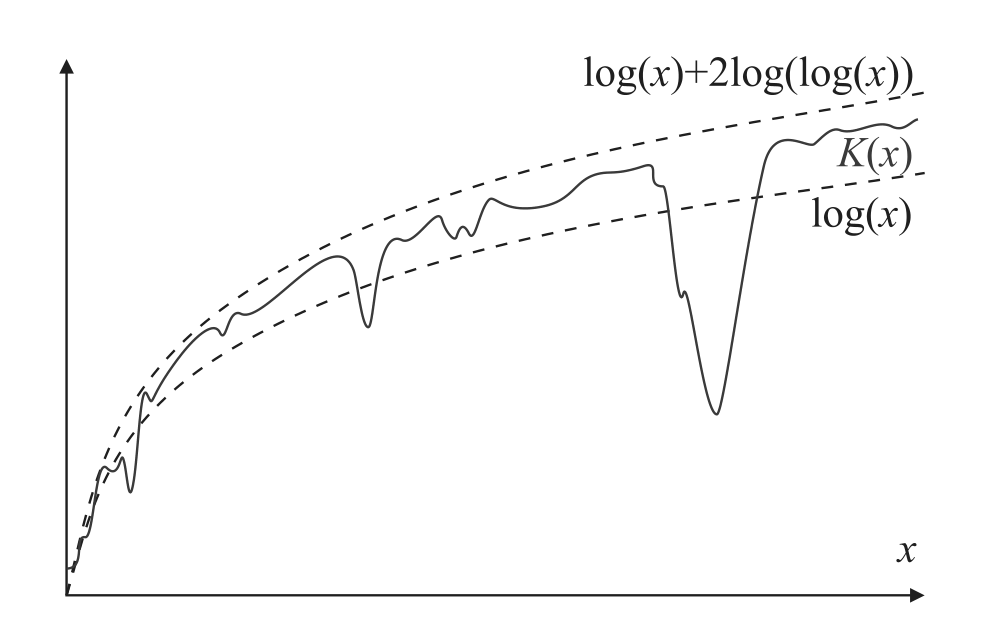
\includegraphics[width=0.5\linewidth]{kcomplexity_graph}
  \end{center}
  \explain{Illustrative graph of prefix Kolmogorov complexity $K(x)$, with
  string $x$ interpreted as an integer on the horizontal axis. By Theorem
  2.7.11, $K(x)\overset{+}{\le}\log_2 x + 2\log_2\log_2 x$ (upper dashed
  curve) for all $x$. By Theorem 2.7.12 (via a counting argument),
  $K(x)\ge \log_2 x$ (lower dashed curve) for ``most'' $x$. The solid
  jagged curve is a schematic of $K(x)$ itself: it generally hugs the
  upper envelope, but has occasional sharp downward plunges at $x$ that
  happen to be very ``simple'' (e.g.\ powers of two, or other structured
  numbers), since those have unusually short programs.}
\end{frame}

\begin{frame}[allowframebreaks]{(In)compressibility and Theorem 2.7.13}
  Now that we have a formal definition of simplicity, we can define a
  string to be \textbf{compressible} if its shortest description is
  shorter than the string itself, i.e.\ $K(x)<\ell(x)$.

  \medskip
  \textbf{Incompressible strings must exist.} By the pigeon-hole
  principle: if all strings were compressible, we could construct an
  injection from $\mathbb{B}^n$ into $\mathbb{B}^{<n}$ (each string mapped
  to its shortest program), which must be injective since running the
  shortest program recovers the original string. But an injection requires
  $|\mathbb{B}^n|\le|\mathbb{B}^{<n}|$, whereas
  $|\mathbb{B}^{<n}|=\sum_{i=0}^{n-1}|\mathbb{B}^i|=\sum_{i=0}^{n-1}2^i=2^n-1<2^n=|\mathbb{B}^n|$
  -- a contradiction.

  \medskip
  This gives no indication of \emph{how common} incompressible strings
  are. Intuitively ``most'' strings should be incompressible: fair coin
  flips are far more likely to look ``random'' than to have an obvious
  pattern such as $101010\ldots$, because simple patterns correspond to
  short programs, of which there are few.

  \framebreak

  \begin{block}{Theorem 2.7.13 (Most strings are incompressible)}
    For any (injective) encoding/compression, less than $2^n$ strings
    $x\in\mathcal{X}^*$ can be compressed to less than $n$ bits. In
    particular, the fraction of strings of length $n$ compressible by more
    than $k$ bits is less than $2^{-k}$. Compressing with a prefix-code
    increases the length of most strings.
    \begin{align*}
      \text{(i)}\quad & 2^{-n}|\{x:\ell(C(x))<n-k\}| < 2^{-k}
        &&\text{for injective } C:\mathcal{X}^*\to\Bstr\\
      \text{(ii)}\quad & 2^{-n}|\{x:\ell(C(x))\le n+k\}| \overset{n\to\infty}{\longrightarrow} 0
        &&\text{for a prefix code } C:\mathcal{X}^*\to\Bstr
    \end{align*}
    In particular both statements hold for $K$-complexity, i.e.\ for
    $\ell(C(x))=K(x)$.
  \end{block}
  \explain{$C$ is any (injective, or prefix-code) compression scheme.
  Statement (i) is the pigeonhole-principle bound made quantitative: the
  \emph{fraction} of length-$n$ strings that can be squeezed into fewer
  than $n-k$ bits is less than $2^{-k}$ -- so ``super-compressible''
  strings become exponentially rare as the savings $k$ grow. Statement
  (ii) says that if you additionally require $C$ to be a valid prefix
  code, then almost none of the strings get compressed at all as
  $n\to\infty$ (a vanishing fraction beat $n+k$ bits) -- so on average, a
  prefix-code compressor makes strings \emph{longer}, not shorter (a
  well-known fact for any real-world compressor: not every input can be
  shrunk).}

  \framebreak

  \small
  \begin{center}
    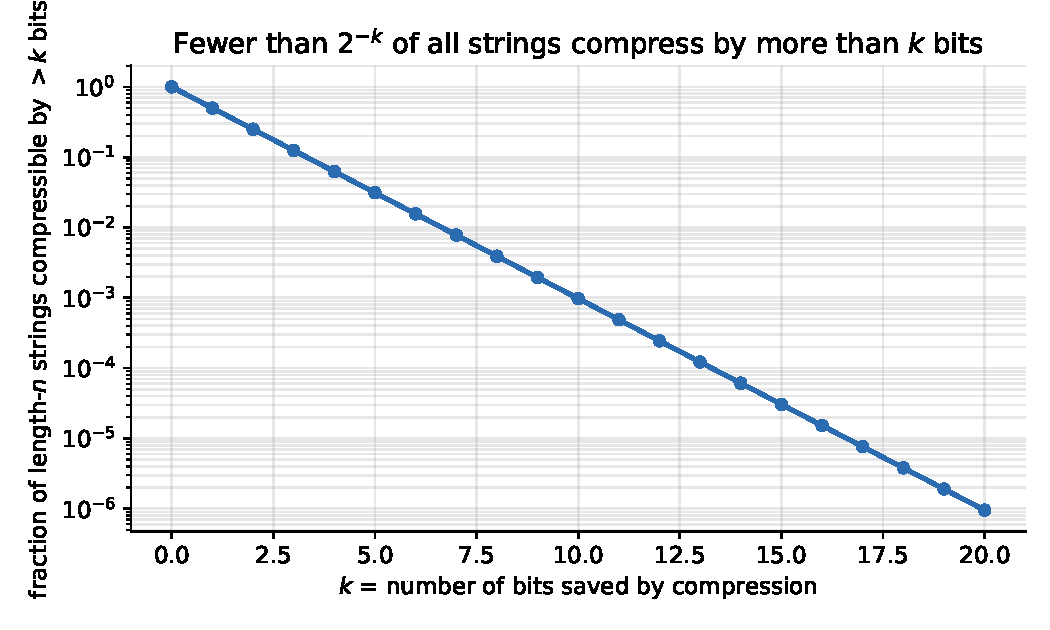
\includegraphics[width=0.62\linewidth]{compressible_fraction}
  \end{center}
  \explain{Plot of the bound $2^{-k}$ from Theorem 2.7.13(i): the
  fraction of length-$n$ strings compressible by more than $k$ bits
  (vertical axis, log scale) shrinks exponentially fast as $k$ grows. For
  example, fewer than 1 in 1024 strings can be compressed by more than 10
  bits, and fewer than 1 in a million can be compressed by more than 20
  bits.}
\end{frame}

\begin{frame}{Definition 2.7.14: Randomness of Individual Sequences}
  \footnotesize
  Incompressibility lets us formally define randomness of \emph{individual}
  strings, dropping the quotation marks around ``random.''
  \begin{block}{Definition 2.7.14 (Randomness of individual sequences)}
    An individual sequence $x_{1:\infty}$ is (called) $\mu$-algorithmically
    random iff one (and hence all) of the following equivalent conditions
    hold:
    \begin{align*}
      \text{(i)}\ & x_{1:\infty} \text{ passes all } \mu\text{-Martin-Löf randomness tests}\\
      \text{(ii)}\ & M(x_{1:n}) \overset{\times}{\le} \mu(x_{1:n}) \ \forall n\\
      \text{(iii)}\ & Km(x_{1:n}) \overset{+}{=} -\log_2\mu(x_{1:n}) \ \forall n\\
      \text{(iv)}\ & K(x_{1:n}) \overset{+}{\ge} -\log_2\mu(x_{1:n}) \ \forall n
    \end{align*}
    For fair coin flips $\mu(x_{1:n})=2^{-n}$, and the qualifier $\mu$- is
    usually dropped.
  \end{block}
  \explain{$\mu$ (mu) is the ``true'' probability measure the sequence is
  supposedly drawn from. $M$ is the universal semimeasure (formally
  introduced in Chapter 3), a Bayes-mixture-style predictor. The
  intuition: a sequence is ``random'' with respect to $\mu$ exactly when
  its Kolmogorov complexity matches what you would expect from a typical
  $\mu$-sample -- i.e.\ its shortest description is about as long as the
  raw information content $-\log_2\mu(x_{1:n})$ (its Shannon
  self-information under $\mu$), meaning it has no shorter, cleverer
  description; there is no exploitable pattern.}
\end{frame}

\begin{frame}[allowframebreaks]{Algorithmic Randomness in Practice}
  Algorithmic randomness can also be defined for \emph{finite} strings
  using the notion of \emph{randomness deficiency}. One can show that a
  finite (infinite) string sampled from $\mu$ is with high probability
  (almost surely) $\mu$-algorithmically random. So while there is no
  algorithm to compute algorithmically random strings, they \emph{can} be
  generated with high probability.

  \medskip
  \textbf{Relation to pseudo-randomness.} A pseudo-random sequence is
  deterministically generated, but no test that runs in polynomial time
  can reliably distinguish it from a sequence sampled from a random
  source. This can be regarded as a practical, poly-time version of
  Martin-Löf randomness tests (which consist of all lower semicomputable
  tests). That is, no constructive test can reliably distinguish an
  algorithmically random sequence from one sampled from a true random
  source.

  \framebreak

  \begin{block}{Theorem 2.7.15 ($K$-complexity tends to infinity)}
    $$\lim_{n\to\infty} K(n) = \infty$$
  \end{block}
  \explain{As $n$ grows without bound, its Kolmogorov complexity is
  eventually forced to grow without bound too -- no infinite subsequence
  of integers can all stay ``simple'' forever.}

  \medskip
  \textbf{Proof.} Suppose not. Then there exists some $N$ such that
  $K(n)<N$ for infinitely many $n$. So infinitely many numbers would have
  Kolmogorov complexity less than $N$, meaning there would be infinitely
  many \emph{programs} of length $<N$ describing them -- but there are
  only finitely many binary strings of length $<N$, a contradiction.

  \medskip
  Returning to properties of $K$, we noted earlier (Figure 2.19) that
  $K(n)\overset{+}{\le}\log_2 n+2\log_2\log_2 n$ for all $n$
  (Theorem 2.7.11), and $K(n)\ge \log_2 n$ for \emph{most} $n$ (Theorem
  2.7.12, since if $K(n)\le\log_2 n$ for a non-vanishing fraction of $n$,
  then $\sum_n 2^{-K(n)}=\infty$, contradicting Theorem 2.7.12). There is
  also some very weak notion of continuity:
  $|K(n\pm k)-K(n)|\overset{+}{\le}K(k)$, so plunges in $K(n)$ for simple
  $n$ have some width. Furthermore, Theorem 2.7.15 implies that the local
  minima of $K$ also increase with $n$, albeit slower than any computable
  function.
\end{frame}

\begin{frame}{Theorem 2.7.16: Extra Information Never Hurts}
  Providing extra side information $y$ can never hurt when trying to
  describe $x$: at worst, $y$ is totally uncorrelated with $x$ and can
  simply be ignored. At best, $y$ is a copy of $x$, so only a constant
  length program is needed to copy the side information to the output.
  Similarly, describing $x$ and $y$ together is at least as hard as
  describing $x$ alone.
  \begin{block}{Theorem 2.7.16 (Extra Information)}
    $$K(x\,|\,y) \;\overset{+}{\le}\; K(x) \;\overset{+}{\le}\; K(x,y)$$
  \end{block}
  \explain{$K(x,y)$ is the Kolmogorov complexity of the pair $(x,y)$
  encoded together as one string. Reading left to right: knowing $y$ can
  only make describing $x$ easier or the same (never harder); and
  describing $x$ alone can only be easier or the same as describing the
  pair $(x,y)$ together.}

  \bigskip
  \textbf{Proof idea.} Let $p^*$ be the shortest program with $U(p^*)=x$.
  A machine that discards the given side information $y'$ and runs $p^*$
  gives $K(x|y)\overset{+}{\le}K(x)$. Let $q^*$ be shortest with
  $U(q^*)=x'y$; a machine that computes $x'y$ from $q^*$ and keeps only
  $x$ gives $K(x)\overset{+}{\le}K(x'y)=K(x,y)$.
\end{frame}

\begin{frame}{Theorem 2.7.17: Subadditivity}
  \small
  Encoding the concatenation $xy$ requires less information than being
  able to encode both $x$ and $y$ separably. This is less information
  still than encoding $x$, along with encoding $y$ given $x$. This is
  less again than encoding $x$, along with encoding $y$ with no help from
  $x$:
  \begin{block}{Theorem 2.7.17 (Subadditivity)}
    $$K(xy) \;\overset{+}{\le}\; K(x,y) \;\overset{+}{\le}\; K(x)+K(y|x) \;\overset{+}{\le}\; K(x)+K(y)$$
  \end{block}
  \explain{$K(xy)$ is the complexity of the raw concatenated string $xy$
  (no separator markers needed, decoder must figure out the split point
  itself, which is even easier than being handed the pair). Each step
  adds a bit more ``help'' for the decoder: (1) knowing $x$ and $y$ can be
  uniquely separated is at least as easy as the raw concatenation, (2)
  which is no harder than an optimal split into ``describe $x$'' plus
  ``describe $y$ given $x$'', which (3) is no harder than describing $x$
  and $y$ completely independently of one another.}

  \bigskip
  \textbf{Proof idea (sketch of 3 parts).} (1) A program for $x'y$ can be
  post-processed by a machine that decodes and discards the separator,
  yielding $xy$ directly. (2) Given the shortest program $q$ for $x$
  (using $U(q)=x$) and the shortest program $r$ for $y$ given $x$ (using
  $U(x'r)=y$), a machine reading $qr$ can uniquely recover $q,r$ (since
  both halt, both are prefix-free) and reconstruct $x'y$. (3) Follows
  since $K(y|x)\overset{+}{\le}K(y)$ by Theorem 2.7.16.
\end{frame}

\begin{frame}[allowframebreaks]{Theorem 2.7.18: Symmetry of Information}
  The following theorem is a bit more difficult to intuit. The idea is
  that the information contained in $y$, together with the minimal
  information to recover $x$ given $y$, should be roughly the same as the
  information contained in $x$, together with the minimal information to
  recover $y$ from $x$.

  \medskip
  \textbf{A restricted intuition.} If $x$ is complex and $y$ is simple,
  then $K(x)$ is large, whereas $K(y|x)\approx 0$ is small (knowing $x$,
  not much more information is required to specify $y$). Conversely,
  $K(y)\approx 0$ is small (as $y$ is simple), but $K(x|y)\approx K(x)$
  (since $y$ is simple, it cannot help much with specifying $x$, as
  otherwise $x$ would also be simple). What is remarkable is that the
  \emph{sum} of these terms, $K(x|y)+K(y)$ and $K(y|x)+K(x)$, are in
  general about equal, regardless of the values of $x$ and $y$.

  \framebreak

  \begin{block}{Theorem 2.7.18 (Symmetry of information)}
    $$K(x\,|\,y,K(y)) + K(y) \;\overset{+}{=}\; K(y\,|\,x,K(x)) + K(x) \;\overset{+}{=}\; K(x,y) \;\overset{+}{=}\; K(y,x)$$
  \end{block}
  \explain{$K(x|y,K(y))$ means ``the complexity of $x$ given both $y$ and
  the number $K(y)$ as side information.'' Equality only holds within a
  logarithmic additive correction (hence the need to also feed in the
  \emph{value} $K(y)$ or $K(x)$, not just $y$ or $x$, as $K(x)$ cannot be
  computed from $x$ alone -- computing $K$ is uncomputable, Theorem
  2.7.27 -- so supplying it as extra side information is genuinely
  helpful).}

  \begin{center}
    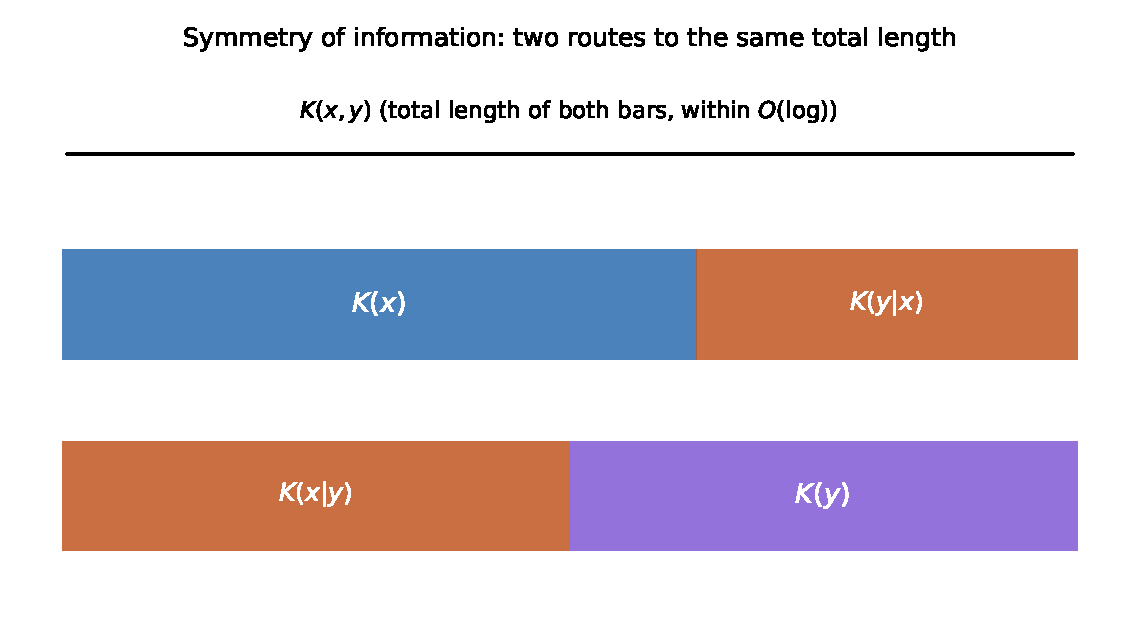
\includegraphics[width=0.72\linewidth]{symmetry_info}
  \end{center}

  \framebreak

  \textbf{Proof idea.} The last equality, $K(x,y)\overset{+}{=}K(y,x)$, is
  easy: given a shortest program $p$ for $x'y$, we can recover $x$ and
  $y$ (using the second-order prefix code), and output $y'x$ instead --
  giving $K(y,x)\overset{+}{\le}K(x,y)$, and symmetrically the reverse, so
  they are equal. Unfortunately, the first two equalities (linking the
  conditional terms) are considerably harder to prove and beyond the
  scope of this course; see the references in the book for a full proof.
\end{frame}

\begin{frame}{Definition 2.7.19: K-Complexity of Computable Functions}
  We have defined Kolmogorov complexity for objects describable as binary
  strings, but mathematical \emph{functions} $f$ require special
  treatment: allowing any formal/axiomatic description of $f$ encoded as
  $\langle f\rangle$ would make $K(\langle f\rangle)$ finite even for
  mathematically describable but \emph{incomputable} functions. Below we
  give a more natural, useful definition restricted to computable
  functions.
  \begin{block}{Definition 2.7.19 (Kolmogorov complexity of computable functions)}
    The Kolmogorov complexity of a computable function
    $f:\Bstr\to\Bstr$ is the length of the shortest program that computes
    $f(x)$ given $x$ as side information:
    $$K(f) \;:=\; \min_{p\in\Bstr}\{\ell(p) : \forall x.\, U(x'p)=f(x)\}$$
  \end{block}
  \explain{$K(f)$ is the shortest \emph{single} program $p$ that, no
  matter which input $x$ you hand it as side information, always
  correctly computes $f(x)$. This captures ``the complexity of the
  algorithm computing $f$'', ignoring what particular input it is run on
  -- unlike encoding a formal mathematical description of $f$, which
  could smuggle in uncomputable functions.}
\end{frame}

\begin{frame}{Definition 2.7.20 and Remark 2.7.21}
  \small
  We also need a custom complexity measure for semi-probability mass
  functions $P$ and semimeasures $\nu$ (nu).
  \begin{block}{Definition 2.7.20 (Complexity of lower semicomputable semimeasures)}
    Let $\mathcal{M}_{sol}=\{\nu_1,\nu_2,\nu_3,\dots\}$ be a canonical
    enumeration of all lower semicomputable semimeasures (Definition
    3.7.1), then the Kolmogorov complexity of $\nu_i$ is defined as
    $$K(\nu_i) \;:=\; K(i) \quad\text{for } \nu_i\in\mathcal{M}_{sol}$$
    The definition of $K(P)$ for lower semicomputable semi-probability
    mass functions is analogous.
  \end{block}
  \explain{Since a semimeasure $\nu$ cannot in general be encoded exactly
  as a finite binary string, we instead identify it by its \emph{index}
  $i$ in a fixed canonical list of all such (lower semicomputable)
  semimeasures, and define $K(\nu_i)$ as simply $K(i)$ -- the complexity
  of that index number.}

  \medskip
  \textbf{Remark 2.7.21 (Confusion of $K(T)$, $K(f)$, $K(\nu)$).}
  $K(f)$ is conceptually different from the Kolmogorov complexity of
  strings and other objects, including Turing machines: many machines $T$
  can compute the same $f$, but some are unnecessarily complicated (e.g.\
  containing a million superfluous never-reached states), so
  $K(T):=K(\langle T\rangle)$ can be far larger than $K(f)$, since $K(f)$
  only encodes the \emph{essence} of $f$ without the ``garbage.'' One
  downside of Definition 2.7.19 is that $K$, as a functional of $f$, is
  itself incomputable (not even approximable). $K(\nu)$ is relative to an
  enumeration of $\mathcal{M}_{sol}$, and is different again.
\end{frame}

\begin{frame}{Theorem 2.7.22: Information Non-Increase}
  \small
  Consider some string $x$, transformed via $f$ into $y=f(x)$. The result
  $y$ cannot be much more complex than a description of the function $f$
  together with the input $x$, since feeding a simple $x$ into a function
  $f$ leads to a complex output $y$ only when $f$ itself is also complex.
  Given a description of both $x$ and $f$, little extra information on
  top is required to describe $f(x)$, as we can simply recover $x$ and
  $f$ from the descriptions, and run $f$ on $x$:
  \begin{block}{Theorem 2.7.22 (Information non-increase)}
    Let $f:\Bstr\to\Bstr$ be a computable function. Then,
    $$K(f(x)) \;\overset{+}{\le}\; K(x) + K(f)$$
  \end{block}
  \explain{Applying a computable function $f$ to a string $x$ can never
  increase the total description length by more than a fixed
  constant beyond $K(x)+K(f)$ -- computation cannot manufacture new
  intrinsic information out of nothing.}

  \bigskip
  \textbf{Proof idea.} Let $q$ be the minimal self-delimiting program
  computing $f$ (per Definition 2.7.19), and $r$ the shortest program with
  $U(r)=x$. There exists an $i$ such that
  $U(i'qr) := U(U(r)'q) = U(x'q) = f(x) =: y$, and since $q,r$ are
  self-delimiting they can be uniquely separated back out of $qr$. So
  $K(f(x))\equiv \min_p\{\ell(p):U(p)=y\}\le \ell(i'qr)\overset{+}{=}
  \ell(q)+\ell(r) = K(f)+K(x)$.
\end{frame}

\begin{frame}[fragile]{Python: Compressors as Practical Upper Bounds on $K(x)$}
  \small
  Since $K$ is not computable (Theorem 2.7.27, coming up), in practice we
  can only get \emph{upper bounds} on it -- any lossless compressor gives
  one, via $K(x)\overset{+}{\le}\ell(C(x))+K(C)$ (Theorem 2.7.9 with $C$
  playing the role of $T$). We check this on our earlier strings $x$
  (periodic), $y$ (digits of $\pi$), $z$ (``random'').
  \begin{lstlisting}
import zlib
x = "10" * 20                                       # periodic, len 40
y = "1100100100001111110110101010001000100001"      # digits of pi, len 40
z = "1011101100110101111100011101011010111011"       # 'random', len 41

for name, s in [("x", x), ("y", y), ("z", z)]:
    raw = int(s, 2).to_bytes((len(s) + 7) // 8, "big")
    print(name, "raw bits =", len(s), " zlib upper bound =",
          len(zlib.compress(raw, level=9)) * 8, "bits")

# Output:  x raw bits = 40  zlib upper bound =  88 bits
#          y raw bits = 40  zlib upper bound = 104 bits
#          z raw bits = 41  zlib upper bound = 112 bits
  \end{lstlisting}
  \explain{At such short lengths, \texttt{zlib}'s fixed header overhead
  dominates and it cannot spot $x$'s or $y$'s pattern, so all three bounds
  are far above the true $K(x)\ll K(y)\approx K(z)$. This is why $K$ is
  only ever \emph{approximable} in practice: a smarter compressor, or a
  much longer version of $x$, would reveal its true low complexity, while
  $z$'s bound would keep growing linearly no matter how clever the
  compressor (Invariance Theorem, Theorem 2.7.6).}
\end{frame}

% =============================================================================
\section{2.7.4 The Minimum Description Length Principle}
% =============================================================================

\begin{frame}{Theorem 2.7.23: The MDL Bound}
  The complexity of $x$ can be bounded above by the complexity of
  encoding some probability distribution $P$, plus $\lceil
  -\log_2P(x)\rceil$, the optimal code length of $x$ with respect to $P$.
  \begin{block}{Theorem 2.7.23 (MDL Bound)}
    If $P:\Bstr\to[0,1]$ is a lower semicomputable semi-probability mass
    function (i.e.\ $\sum_{x\in\Bstr}P(x)\le 1$) and $\mu$ a lower
    semicomputable semimeasure (Definition 2.2.11), then
    $$K(x) \overset{+}{\le} -\log_2 P(x) + K(P)
    \qquad\text{and}\qquad
    Km(x) \overset{+}{\le} -\log_2\mu(x) + K(\mu)$$
  \end{block}
  \explain{MDL stands for \emph{Minimum Description Length}. This says:
  the complexity of $x$ is at most the cost of specifying a distribution
  $P$ (i.e.\ $K(P)$ bits), plus the Shannon-optimal code length of $x$
  under that distribution ($-\log_2P(x)$ bits, per the Shannon-Fano coding
  results of Section 2.5). Intuitively: describe a good \emph{model} for
  $x$, then describe $x$ using that model -- a ``two-part code.''}

  \medskip
  \textbf{Proof sketch (first bound).} Using a Shannon-Fano code based on
  $P$: let $s_x:=\lceil-\log_2P(x)\rceil$. By Kraft's inequality
  (Theorem 2.5.17) there is a prefix code $c$ with $\ell(c(x))=s_x$. A
  machine reading a program for $P$ (length $K(P)$) plus the codeword
  $c_x$ recovers $x$, giving
  $K(x)\le \ell(i'c_xp^*) \overset{+}{=} -\log_2P(x)+K(P)$.
\end{frame}

\begin{frame}{Definition 2.7.24: The MDL Principle}
  The MDL bound is useful for proving other theorems, but its most
  important application is in \textbf{model selection}: Occam's razor
  demands selecting the simplest theory/model consistent with the data,
  which can be quantified as: the best explanation of $x$ is the shortest
  program $p^*$ on a universal Turing machine $U$ for which $U(p^*)=x$.
  \begin{block}{Definition 2.7.24 (The Minimal Description Length (MDL) Principle)}
    Given a class of probability distributions $\mathcal{M}$ and data $x$,
    the MDL principle selects the model with the shortest two-part code:
    $$Q^{\text{MDL}} \;:=\; \operatorname*{arg\,min}_{Q\in\mathcal{M}}\{-\log_2 Q(x)+K(Q)\}$$
  \end{block}
  \explain{$Q^{\text{MDL}}$ is the model chosen by the MDL principle:
  among all candidate models $Q$ in a class $\mathcal{M}$, pick the one
  that minimizes ``bits to describe the model'' plus ``bits to describe
  the data using that model.'' This gives Theorem 2.7.23 its name. Under
  very mild conditions, one can prove that the MDL estimator is
  consistent (i.e.\ converges to the true model as data grows).}
\end{frame}

\begin{frame}[allowframebreaks]{Parametric MDL and the Bayesian Derivation}
  In practice, we must replace $K(Q)$ with more easily computable upper
  bounds. For instance, if $\mathcal{M}=\bigcup_{d=0}^\infty\mathcal{M}_d$
  where $\mathcal{M}_d$ is a class of i.i.d.\ distributions from which
  $x=x_{1:n}$ is sampled (e.g.\ polynomials of degree $d-1$ with Gaussian
  noise), smoothly parameterized by some $\theta\in\mathbb{R}^d$, then MDL
  becomes
  \begin{equation*}
  Q^{\text{MDL}} := \operatorname*{arg\,min}_{d\in\mathbb{N}_0,\,\theta\in\mathbb{R}^d}
  \left\{-\log_2 Q_\theta(x) + \tfrac{d}{2}\log_2 n + O(d)\right\} \tag{2.7.25}
  \end{equation*}
  \explain{$\theta$ (theta) is the parameter vector of the model (e.g.\
  polynomial coefficients), $d$ is the number of parameters (model
  ``size''/degrees of freedom), and $n$ is the sample size. Intuitively,
  for sample size $n$, each parameter $\theta_i$ can only be estimated to
  accuracy $O(1/\sqrt n)$, so only the first
  $\log_2[1/O(1/\sqrt n)]=\tfrac12\log_2 n+O(1)$ bits of the expansion of
  each parameter need to be encoded -- hence the $\tfrac{d}{2}\log_2 n$
  penalty term for a $d$-parameter model.}

  \medskip
  The $O(d)$ term depends on the smoothness of the parametrization, and
  can be explicitly quantified as $\log_2\int\sqrt{\det[\mathcal{I}(\theta)/2\pi
  e]}\,d^d\theta$, where $\mathcal{I}(\theta)$ is the Fisher Information
  Matrix of $Q_\theta$ (Definition 2.3.12, generalized to $\theta\in\mathbb{R}^d$
  by replacing $\partial$ with $\nabla$ (nabla, the gradient)). The
  dominant term $-\log_2Q_\theta(x)$ is linear in $n$; the Bayesian
  Information Criterion (BIC) penalty $\tfrac{d}{2}\log_2 n$ is
  logarithmic in $n$; while $O(d)$ is a small correction that may be
  neglected.

  \framebreak

  \textbf{Bayesian derivation.} The same expression can be derived from
  Bayesian principles. In the discrete case, MDL approximates the full
  Bayesian mixture $\sum_{Q\in\mathcal{M}}Q(x)w(Q)$ (replace the sum by a
  max, take the logarithm, change sign, choose prior $w(Q)=2^{-K(Q)}$,
  and this recovers Definition 2.7.24 exactly). In the parametric
  continuous case, with priors $w_d(\theta)$ over the parameters, the
  \emph{Maximum A Posteriori} (MAP) approximation is
  \begin{equation*}
  Q^{\text{MAP}} := \operatorname*{arg\,max}_{\theta\in\mathbb{R}^{d^*}}
  \{Q_\theta(x)w_{d^*}(\theta)\}, \quad\text{where}\quad
  d^* := \operatorname*{arg\,max}_{d\in\mathbb{N}_0}\left\{\int
  Q_\theta(x)w_d(\theta)\,d^d\theta\right\} \tag{2.7.26}
  \end{equation*}
  \explain{Using Laplace approximation for the integral for large $n$,
  and taking the negative logarithm, (2.7.26) reduces to (2.7.25). If we
  choose the reparameterization-invariant, minimax-optimal
  Jeffreys/Bernardo prior (Definition 2.4.11) for $w_d(\theta)$, then even
  the $O(d)$ term coincides between Bayes and MDL. In the continuous
  case, Bayes and MDL differ only in $o(1)$ terms that vanish as
  $n\to\infty$.}

  \framebreak

  \textbf{Regularization in Machine Learning (RML).} MDL can also be
  understood as a \emph{Penalized/Regularized Maximum Likelihood (RML)}
  principle -- maximizing $Q(x)$ is the same as minimizing $-\log_2Q(x)$,
  but punishing complex models by adding $K(Q)$. More generally,
  regularization in classical machine learning combats overfitting to a
  too-complex model by adding a regularization term to the loss function.

  \medskip
  \textbf{Differences between MDL and RML:}
  \begin{itemize}
    \item MDL (Definition 2.7.24) is completely general: it makes no
      assumption whatsoever on the underlying model class $\mathcal{M}$
      (no i.i.d.\ or stationarity or ergodicity or parametric or
      smoothness assumptions), while RML is somewhat tailored towards
      i.i.d.\ data.
    \item MDL is limited to log-loss, while any loss can be used in RML.
    \item RML requires choosing a penalty and tuning its strength (often
      by cross-validation), while MDL theory dictates the penalty.
    \item MDL estimates probabilities $Q$, while RML determines mappings
      $f$ -- though this difference is superficial, since one can
      trivially generalize $Q(x)$ to $Q(y|x)$ in MDL, and augment $f$
      with a noise model in RML.
  \end{itemize}
\end{frame}

\begin{frame}[fragile]{Python: MDL Model Selection -- Occam's Razor in Action}
  \footnotesize
  Fit polynomials of increasing degree to noisy data; use the parametric
  MDL score (2.7.25) to pick the best degree.
  \vspace{-0.3em}
  \begin{lstlisting}
import numpy as np
rng = np.random.default_rng(0)
n = 30
x_pts = np.linspace(-1, 1, n)
true_y = 0.5 + 1.5 * x_pts - 0.8 * x_pts**2      # true model has degree 2
y_pts = true_y + rng.normal(scale=0.15, size=n)  # add Gaussian noise

def mdl_score(degree):
    d = degree + 1                               # number of parameters
    coeffs = np.polyfit(x_pts, y_pts, degree)
    sse = np.sum((y_pts - np.polyval(coeffs, x_pts)) ** 2)
    sigma2 = sse / max(n - d, 1)                 # unbiased noise estimate
    neg_log_lik = 0.5 * n * np.log2(2 * np.pi * sigma2 * np.e)  # -log2 Q(x)
    return neg_log_lik + 0.5 * d * np.log2(n)    # + d/2 * log2(n) penalty

# degree:   0      1      2       3       4       5       6       7
# MDL(bits): 61.40   9.76 -20.96  -19.04  -17.90  -18.04  -18.92  -15.77
#                    ^-- minimum: MDL correctly picks the true degree (2)
  \end{lstlisting}
  \explain{Each extra coefficient reduces the fit error, but costs an
  extra $\tfrac12\log_2 n$ bits under the BIC penalty of (2.7.25). MDL
  correctly identifies degree 2 (the true model) as the global minimum:
  beyond it, the parameter penalty outweighs the tiny fit improvement --
  Occam's razor made quantitative.}
\end{frame}

% =============================================================================
\section{2.7.5 Approximating K-Complexity}
% =============================================================================

\begin{frame}{Approximating $K$: What Can and Cannot Be Done}
  The Kolmogorov complexity $K$ is a universal complexity measure, in
  that $K$ will pick up any regularity or pattern in the data, and use it
  to give as short as possible a description of the input. Viewed
  another way, $K(x)$ provides an absolute limit on the fewest number of
  bits required to express $x$, when compressed by an optimal compressor:
  it beats all other lossless compressors in terms of space saved.

  \medskip
  Unfortunately (though it shouldn't come as a surprise), $K$ is
  \textbf{incomputable}.
\end{frame}

\begin{frame}{Theorem 2.7.27: K Is Not Finitely Computable}
  \begin{block}{Theorem 2.7.27 ($K$ is not finitely computable)}
    $$K \notin \Delta_1^0$$
  \end{block}
  \explain{$\Delta_1^0$ (delta-one-zero) is the class of computable
  functions/decision problems from Section 2.6's arithmetical hierarchy.
  This theorem says there is no algorithm that, given any string $x$,
  always halts and outputs the exact value $K(x)$.}

  \bigskip
  \textbf{Proof.} Assume $K$ is finitely computable. Define
  $f(m):=\min\{n : K(n)\ge m\}$, well-defined since $K$ is unbounded
  (Theorem 2.7.15). Since $K$ is assumed computable, $f$ is also
  computable (compute $K(n)$ for increasing $n$ until $K(n)\ge m$). By
  definition, $K(f(m))\ge m$. By Theorem 2.7.22, $K(f(m))\le K(m)+K(f)+c_1$,
  and by Theorem 2.7.11, $K(m)\le \log_2 m+2\log_2\log_2 m+c_2\le
  2\log_2 m+c_3$. Combining,
  $$m \le K(f(m)) \le K(m)+K(f)+c_1 \le 2\log_2 m + K(f) + c_1+c_3$$
  which gives $m\le 2\log_2 m+O(1)$ for \emph{all} $m$ -- a contradiction,
  since $\log_2 m$ grows far slower than $m$.
\end{frame}

\begin{frame}{Theorem 2.7.28: K Is Upper Semicomputable}
  Not all is lost: we can still approximate $K$ in the limit from above
  (it is upper semicomputable), obtaining better and better upper bounds
  for the complexity of a string.
  \begin{block}{Theorem 2.7.28 ($K$ is upper semicomputable)}
    $$K \in \Pi_1^0$$
  \end{block}
  \explain{Upper semicomputable (recall Section 2.6) means there is an
  algorithm that computes a decreasing sequence of upper bounds
  converging to $K(x)$ in the limit -- we can get arbitrarily close from
  above, we just never know for certain how close we currently are.}

  \bigskip
  \textbf{Construction idea.} We start with some initial program $p_0$
  that simply prints $x$ (a hardcoded copy), giving an initial upper
  bound $C=\ell(x)+2\log_2\ell(x)+O(1)$. We then search over all programs
  $p$ shorter than $p_0$, running them ``in parallel.'' If any program
  $p$ prints $x$ and halts, and is shorter than the best found so far, we
  update $C:=\ell(p)$. Eventually we must stumble across the true shortest
  program $p^*$ and obtain $C=K(x)$ -- but we can never know \emph{when}
  we've found it (the halting problem, Theorem 2.6.7), since some
  not-yet-halted programs might still halt and print $x$ if left to run
  long enough.
\end{frame}

\begin{frame}{Running Infinitely Many Machines at Once: Dovetailing}
  \footnotesize
  We can simulate a whole family of Turing machines ``in parallel'' on a
  single Turing machine, via \textbf{dovetailing}: take an effective
  enumeration $\{T_1,T_2,\dots\}$ of all Turing machines, and timeshare
  according to the schedule $1,2,1,3,1,2,1,4,1,2,1,3,1,2,1,5,\dots$ (half
  of all time to $T_1$, a quarter to $T_2$, an eighth to $T_3$, \dots).

  \begin{center}
    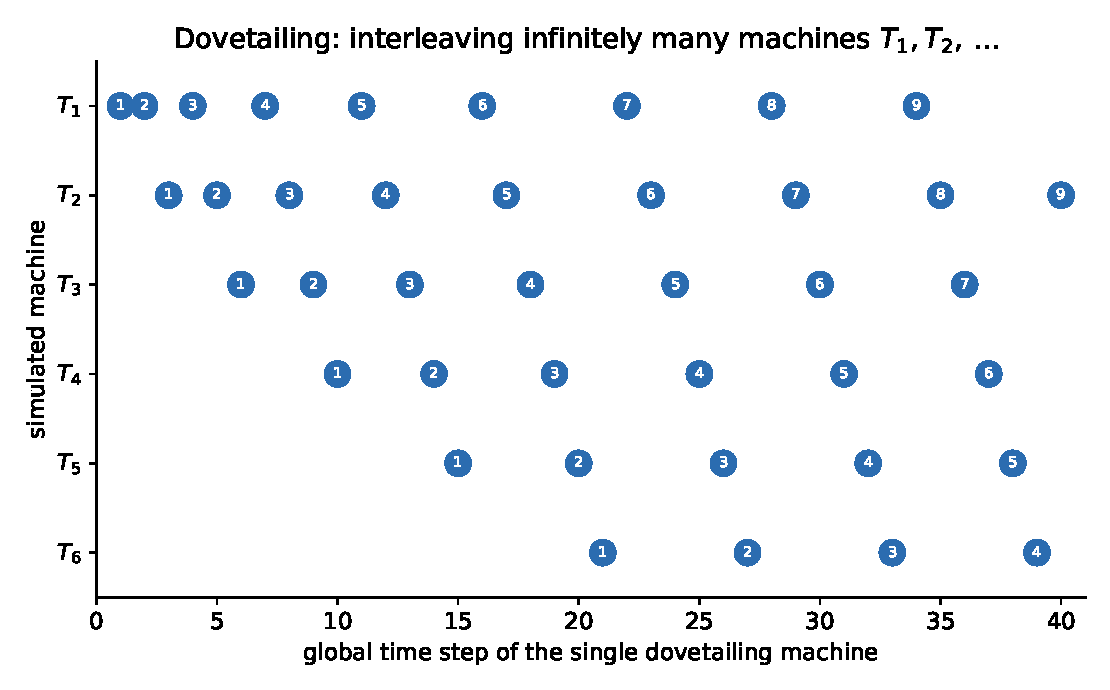
\includegraphics[width=0.42\linewidth]{dovetail}
  \end{center}
  \explain{Each dot shows, at a global time step (horizontal axis) of the
  ``master'' machine, which simulated machine $T_i$ (vertical axis) is
  advanced; the number inside is that machine's own local step count. As
  a corollary, we can also run finitely many machines the same way,
  idling on any step not assigned to a listed machine.}
\end{frame}

\begin{frame}{Proof Sketch of Theorem 2.7.28}
  To prove $K$ is upper semicomputable, we describe a finitely computable
  function $\phi:\Bstr\times\mathbb{N}_0\to\mathbb{N}_0$ such that
  $\lim_{t\to\infty}\phi(x,t)=K(x)$ and $\phi(x,t)\ge\phi(x,t+1)$
  (monotonically non-increasing).

  \medskip
  \textbf{Algorithm for $\phi$.}
  \begin{enumerate}
    \item Initialize $C:=\lceil \ell(x)+2\log_2\ell(x)+\ell(i')\rceil$,
      where $i'$ is the index of a Turing machine decoding second-order
      prefix codes (by Theorem 2.7.11, $C$ is an upper bound for $K(x)$).
    \item Dovetail $U(p_i)$ for all prefix programs $p_1,p_2,\dots$ for
      $t$ time steps. Every time some simulation $U(p_i)$ halts and
      outputs $x$, let $C:=\min\{C,\ell(p_i)\}$ (which can only ever make
      $C$ smaller, while still being an upper bound for $K(x)$).
    \item Once $t$ time steps have been simulated, abort the dovetail
      procedure and return $C$.
  \end{enumerate}
  \explain{Allowing this algorithm to run for more time can only make the
  output smaller, so $\phi(x,t)\ge\phi(x,t+1)$. For every $x$ there
  exists a shortest program $p$ with $K(x)=\ell(p)$, so by running the
  dovetailing procedure long enough, we will eventually stumble across
  this shortest program, run it for long enough to confirm $U(p)=x$, and
  hence $\lim_{t\to\infty}\phi(x,t)=K(x)$, as required.}
\end{frame}

% =============================================================================
\section{2.7.6 Relation to Shannon Entropy}
% =============================================================================

\begin{frame}{Table 2.20: K-Complexity vs.\ Shannon Entropy}
  \footnotesize
  We compare properties of $K$-complexity with those of Shannon entropy:
  many properties of $K$-complexity have an analogous Shannon-entropy version.
  \begin{center}
  \renewcommand{\arraystretch}{1.05}
  \begin{tabular}{@{}p{0.9cm}p{2.1cm}p{5.2cm}p{4.4cm}@{}}
    \toprule
    \textbf{Thm.} & \textbf{Name} & \textbf{Kolmogorov Complexity} & \textbf{Shannon Entropy} \\
    \midrule
    2.7.11 & Upper bound & $K(x)\overset{+}{\le}\ell(x)+2\log_2\ell(x)$ & $H(X)\le \log_2|\mathcal{X}|$ \\
    2.7.16 & Extra Info. & $K(x|y)\overset{+}{\le}K(x)\overset{+}{\le}K(x,y)$ & $H(X|Y)\le H(X)\le H(X,Y)$ \\
    2.7.17 & Subadditivity & $K(x,y)\overset{+}{\le}K(x)+K(y)$ & $H(X,Y)\le H(X)+H(Y)$ \\
    2.7.18 & Symm.\ of Info. & \scriptsize$K(x|y,K(y))+K(y)\overset{+}{=}$\newline\scriptsize$K(y|x,K(x))+K(x)\overset{+}{=}K(x,y)$ & \scriptsize$H(X|Y){+}H(Y){=}H(X,Y)$\newline\scriptsize$=H(Y|X){+}H(X)$ \\
    2.7.22 & Info.\ Non-incr. & $K(f(x))\overset{+}{\le}K(x)+K(f)$ & $H(f(X))\le H(X)$ \\
    2.7.23 & MDL Bound & $K(x)\overset{+}{\le}-\log_2 Q(x)+K(Q)$ & $H(X)\le \mathbb{E}_P[-\log_2 Q(X)]$ \\
    \bottomrule
  \end{tabular}
  \end{center}
  \explain{$x,y$ are strings; $X\sim P,\,Y\sim Q$ are random variables;
  $f$ is a computable function. Every $K$-complexity inequality about
  \emph{strings} has a direct counterpart about the \emph{expected} code
  length of \emph{random variables}, up to an additive $O(1)$ (for $K$)
  vs.\ an exact (in)equality (for $H$, which has no fudge-factor since it
  is an expectation, not tied to any one reference machine).}
\end{frame}

\begin{frame}{Remark 2.7.29: Further Conditioning}
  \begin{block}{Remark 2.7.29 (Further conditioning)}
    Results for Shannon entropy, valid for some probability distribution
    $P(\cdot|\cdot)$, naturally also hold for $P(\cdot|\cdot,Z)$ further
    conditioned on some $Z$. The analogue for $K$-complexity is to
    condition $K$ on a further string $z$, by providing $z$ on an extra
    tape or concatenating it with $y$ or as an oracle. That is, all the
    results above remain valid if conditioning $K$ (further) on some $z$.
  \end{block}
  \explain{This is a ``for free'' extension: every inequality in Table
  2.20 still holds if you imagine every term additionally conditioned on
  some common extra piece of information $z$ (or $Z$ for the random
  variable case) -- e.g.\ $K(x|z) \overset{+}{\le} \ell(x)+2\log_2\ell(x)$
  given $z$ as side information on an extra tape, and so on for every
  other row of the table.}
\end{frame}

% =============================================================================
\section{2.7.7 Exercises}
% =============================================================================

\begin{frame}[allowframebreaks]{Section 2.7.7: Exercises (Overview)}
  The chapter closes with exercises that reinforce the machinery built up
  in this section:
  \begin{enumerate}
    \item Prove the two claims in Definition 2.7.1: that the set of
      halting programs for a prefix TM is prefix-free, and that the set
      of programs producing a given output prefix for a monotone TM is
      prefix-free.
    \item Show that, for $P(x):=\mu(x)$ on strings of length $n$, the
      optimal code length bound $\ell(C(x))>-\log_2P(x)+\log_2\delta$
      holds with probability at least $1-\delta$ (delta) -- a
      high-probability lower bound on $K(x_{1:n})$.
    \item Fill in the details of the proof of Theorem 2.7.23 (the second,
      arithmetic-coding-based MDL bound for semimeasures).
    \item Strengthen Theorem 2.7.28: prove there is no unbounded
      \emph{computable} lower bound to $K$, i.e.\ $f(m):=\min_{n\ge
      m}K(n)$ grows incomputably slowly.
    \item Define the \emph{normalized compression distance}
      $$d(x,y) := \frac{\max\{K(y|x),K(x|y)\}}{\max\{K(x),K(y)\}}$$
      and prove that (within additive constants) $d$ is a metric on
      $\Bstr$.
    \item Show that for every string $x$ there exists a universal Turing
      machine $U'$ such that $K_{U'}(x)=1$ (cf.\ Example 2.7.5), and
      argue why $U'$ cannot be a ``natural'' reference machine if $x$ is
      complex.
  \end{enumerate}
  \explain{$\delta$ (delta) here denotes a small failure probability, as
  is standard in probabilistic bounds. These exercises deepen the same
  themes covered on the preceding slides: prefix-freeness, high
  probability bounds, incomputability limits, and the use of $K$ as a
  similarity/distance measure between objects.}
\end{frame}

% =============================================================================
\section{Summary}
% =============================================================================

\begin{frame}{Chapter Summary: Kolmogorov Complexity}
  \begin{itemize}
    \item \textbf{Motivation.} Shannon entropy measures expected
      information of a \emph{source}; Kolmogorov complexity $K(x)$
      measures the intrinsic information of a single \emph{object} $x$,
      via the length of its shortest program on a fixed universal Turing
      machine $U$.
    \item \textbf{Invariance.} The choice of ``natural'' UTM only matters
      up to an additive constant (Theorem 2.7.6) -- but can be made
      arbitrarily biased if chosen adversarially (Example 2.7.5).
    \item \textbf{Core properties.} Upper bound
      ($K(x)\overset{+}{\le}\ell(x)+2\log_2\ell(x)$), Kraft's inequality,
      extra information, subadditivity, and symmetry of information all
      mirror analogous Shannon entropy results (Table 2.20).
    \item \textbf{Incompressibility \& randomness.} Most strings are
      incompressible (Theorem 2.7.13); this underlies the formal
      definition of algorithmic randomness of individual sequences
      (Definition 2.7.14).
    \item \textbf{MDL Principle.} Occam's razor made rigorous: pick the
      model minimizing description length of model + data given model
      (Definition 2.7.24), connecting to Bayesian MAP estimation and BIC.
    \item \textbf{Incomputability.} $K$ cannot be computed exactly
      (Theorem 2.7.27), but can be approximated arbitrarily well from
      above via dovetailing (Theorem 2.7.28) -- every practical compressor
      gives such an upper bound.
  \end{itemize}
\end{frame}

\end{document}
